% CityFlow coursework report based on the supplied Games Engineering template.
% Replace the two author placeholders before submission.

\documentclass[10pt, a4paper, twocolumn]{article}

\usepackage{GamesEngineering}
\usepackage{tikz}
\usetikzlibrary{arrows.meta,positioning}
\usepackage[hidelinks]{hyperref}

\title{CityFlow: Procedural Road Generation for a Traffic Planning Game}

\author{
    \authorstyle{[YOUR NAME]}
    \newline
    \authorstyle{[YOUR STUDENT ID]}
    \newline\newline
    \institution{}
}

\date{\today}

\begin{document}

\maketitle
\thispagestyle{firstpage}

\lettrineabstract{CityFlow is a road-planning and traffic-simulation game made in Unreal Engine 5.6. The player designs a road network and can ask a procedural generator for one simple possible solution. The main feature comes from my critical review of procedural road generation and L-systems. This report explains the game design, technical structure, critical feature, and testing process.}

\section{Short GDD}

\subsection{Core mechanics}

CityFlow is a strategy game with three phases: Planning, Simulation, and Evaluation. During Planning, buildings are placed on a grid and the player designs the road network. The left mouse button places roads and the right mouse button removes them. Each road tile uses part of a limited shared budget. Road meshes automatically change into straight roads, corners, T-junctions, or crossroads according to their neighbours.

The automatic road generator is not designed only to create smaller branches. It acts as an assistant when the player is unsure how to continue. It studies building entrances, existing roads, obstacles, and the remaining budget, then provides one simple possible solution for connecting the city. The result is not always the most efficient network. Its purpose is to open the player's thinking and provide an example that can be studied and improved. Procedural generation therefore supports the player's decisions instead of replacing them.

During Simulation, road editing is disabled and vehicles travel between buildings using A* pathfinding and spline movement. They queue behind traffic and request access before entering busy intersections. Moving the cursor over a vehicle highlights it and displays an arrow towards its destination. A normal vehicle explodes if it remains blocked for longer than its waiting limit. A Rampage vehicle instead goes out of control, moves faster, ignores normal traffic restrictions, and destroys vehicles in its path. A Teleport vehicle jumps forward along its planned route when its waiting limit is reached, but it may destroy another vehicle if the destination area is occupied.

\begin{figure}
    \centering
    \includegraphics[width=\linewidth]{\detokenize{images/Main gameplay overview.png}}
    \caption{Planning view with buildings, grid cells, arterial roads, budget, and PCG control.}
    \label{fig:overview}
\end{figure}

Figure~\ref{fig:overview} shows the main planning view. The player must connect every building, but connection alone is not enough. A poor network can create long routes, heavy congestion, and more vehicle deaths. Random Mode therefore provides Easy, Medium, and Hard settings. Higher settings add more buildings and faster vehicle spawning, while budget per building becomes lower.

The main source of engagement is the balance between planning and uncertainty. The generator gives a simple answer when the player is stuck, but the player must judge whether that answer uses the budget well and can support dense traffic. Evaluation reports building connectivity, successful arrivals, vehicle deaths, travel efficiency, road-budget use, and runtime. Random maps and unexpected vehicle events make each city different while keeping the player's choices important.

\subsection{Narrative}

The player acts as a planner in a growing modern city. Residential and commercial buildings must join one shared road system. Each match represents a different attempt to balance planned infrastructure with uncertain traffic behaviour.

\subsection{Art style}

The art style uses colourful low-poly models, grey modular roads, and a clear top-down camera. Buildings, vehicles, roads, and feedback markers use strong colour differences so traffic remains readable when the city becomes busy. This style was also realistic for the project schedule.

\subsection{Player support}

Player support includes a data-driven tutorial, English and Simplified Chinese localisation, master and SFX volume settings, placement sounds, score popups, vehicle warnings, and a detailed final report. These systems meet the brief's need for in-game help and player feedback.

\begin{figure*}[t]
    \centering
    \begin{minipage}[t]{0.31\textwidth}
        \centering
        \includegraphics[height=3.2cm,width=\linewidth,keepaspectratio]{\detokenize{images/Difficulty selection.png}}\\[-1mm]
        \footnotesize (a) Difficulty information
    \end{minipage}\hfill
    \begin{minipage}[t]{0.31\textwidth}
        \centering
        \includegraphics[height=3.2cm,width=\linewidth,keepaspectratio]{\detokenize{images/TutorialWidget.png}}\\[-1mm]
        \footnotesize (b) Data-driven tutorial
    \end{minipage}\hfill
    \begin{minipage}[t]{0.31\textwidth}
        \centering
        \includegraphics[height=3.2cm,width=\linewidth,keepaspectratio]{\detokenize{images/Final evaluation report.png}}\\[-1mm]
        \footnotesize (c) Evaluation report
    \end{minipage}
    \caption{The UI explains match settings, teaches the game, and reports results.}
    \label{fig:ux}
\end{figure*}

\section{Short TDD}

\subsection{Architecture}

\texttt{CityFlowGameMode} controls the three gameplay phases. \texttt{GridManager} stores cell types, road connections, and budget. \texttt{LSystemManager} builds PCG roads. \texttt{VehicleManager} spawns vehicles and finds routes. \texttt{ScoringManager} records results. \texttt{CityFlowHUD} manages menus and feedback. Unreal delegates pass important events between these systems, which reduces direct references.

The grid is a two-dimensional cell array. Each cell records whether it is empty, road, or building. It also stores a four-direction connection mask. Road actors use this mask to select a mesh and rotation. Buildings can cover several cells and rotate in 90-degree steps. Their entrances are stored in local grid space and transformed after rotation. Procedural meshes create rounded foundations and sidewalks around each footprint.

\subsection{Key systems}

\paragraph{PCG road system.}

L-systems use repeated production rules to create complex structures from simple symbols \citep{prusinkiewicz1990}. Parish and M\"uller used an extended L-system to produce street networks and buildings \citep{parish2001}. Later work added interactive control to procedural street modelling \citep{chen2008}. These ideas informed the first CityFlow prototype.

A pure local rule system caused a gameplay problem. Organic roads looked useful, but they did not always connect every building into one network. CityFlow therefore uses a hybrid method. First, it finds the main road component. It searches from unconnected entrances and reserves enough budget for complete connection paths. Existing roads have zero extra cost, so they are reused. Candidate connection steps are scored by distance and direction towards useful entrances, with controlled randomness. The player-facing goal is to present one understandable possible answer, not to claim that the generated layout is the best solution.

\begin{figure*}[t]
    \centering
    \begin{minipage}[t]{0.32\textwidth}
        \centering
        \includegraphics[height=3.0cm,width=\linewidth,keepaspectratio]{\detokenize{images/arterial roads before generation.png}}\\[-1mm]
        \footnotesize (a) Player arterial roads
    \end{minipage}\hfill
    \begin{minipage}[t]{0.32\textwidth}
        \centering
        \includegraphics[height=3.0cm,width=\linewidth,keepaspectratio]{\detokenize{images/L-system growth in progress.png}}\\[-1mm]
        \footnotesize (b) PCG growth
    \end{minipage}\hfill
    \begin{minipage}[t]{0.32\textwidth}
        \centering
        \includegraphics[height=3.0cm,width=\linewidth,keepaspectratio]{\detokenize{images/Final network showing all building.png}}\\[-1mm]
        \footnotesize (c) Connected result
    \end{minipage}
    \caption{The hybrid PCG process uses the player's roads to present one possible connected solution.}
    \label{fig:pcg}
\end{figure*}

Figure~\ref{fig:pcg} shows the main PCG stages. This approach keeps visible variety but gives a clearer gameplay goal. It also follows the wider PCG aim of creating useful game content within design constraints \citep{hendrikx2013}.

\paragraph{Traffic simulation.}

Vehicles use A* over connected road cells. Grid paths become world-space splines with lane offsets. Forward probes detect vehicles ahead. T-junctions and crossroads use direction-based reservations, so conflicting traffic does not enter at the same time. Hover feedback highlights a vehicle and shows its destination direction. A normal vehicle explodes after a long wait. Rampage vehicles instead ignore probes and junction reservations, accelerate, and destroy vehicles in their path. Teleport vehicles jump forward along their current spline and destroy overlapping vehicles at the landing position. These different timeout results make serious congestion visible and affect the evaluation score.

\begin{figure*}[t]
    \centering
    \begin{minipage}[t]{0.31\textwidth}
        \centering
        \includegraphics[height=3.2cm,width=\linewidth,keepaspectratio]{\detokenize{images/traffic during Simulation.png}}\\[-1mm]
        \footnotesize (a) Traffic during Simulation
    \end{minipage}\hfill
    \begin{minipage}[t]{0.21\textwidth}
        \centering
        \includegraphics[height=3.2cm,width=\linewidth,keepaspectratio]{\detokenize{images/Intersection reservation indicator.png}}\\[-1mm]
        \footnotesize (b) Junction state
    \end{minipage}\hfill
    \begin{minipage}[t]{0.21\textwidth}
        \centering
        \includegraphics[height=3.2cm,width=\linewidth,keepaspectratio]{\detokenize{images/vehicle with outline and destination arrow.png}}\\[-1mm]
        \footnotesize (c) Vehicle inspection
    \end{minipage}\hfill
    \begin{minipage}[t]{0.21\textwidth}
        \centering
        \includegraphics[height=3.2cm,width=\linewidth,keepaspectratio]{\detokenize{images/SpecialVehicle.png}}\\[-1mm]
        \footnotesize (d) Special vehicles
    \end{minipage}
    \caption{Traffic flow, junction reservations, vehicle inspection feedback, and special timeout behaviours.}
    \label{fig:traffic}
\end{figure*}

\subsection{Libraries and tools used}

Unreal Engine modules provide the main reusable systems. Enhanced Input handles camera and placement controls. Niagara provides explosion and teleport effects. ProceduralMeshComponent builds foundations and sidewalks at runtime. UMG and Slate support menus and HUD widgets. Data Assets store configurable buildings, vehicles, and tutorial entries. Sound Classes group master audio and SFX, while Unreal's localisation pipeline provides English and Simplified Chinese. Git LFS stores the binary Unreal assets used by the project.

\section{Technical Overview}

\textbf{Tools:} Unreal Engine 5.6, Visual Studio 2022, Git, and Git LFS. \textbf{Programming languages:} C++ for runtime systems and Unreal Blueprints for asset configuration and presentation. \textbf{Target platform:} Windows desktop using DirectX 12. The game is developed and tested as a native Unreal Engine application.

The source project, setup instructions, dependencies, and asset notes are available at \href{https://github.com/zhenyanlong/CityFlow}{\texttt{zhenyanlong/CityFlow}}. A packaged Windows executable is provided through the repository's \href{https://github.com/zhenyanlong/CityFlow/releases}{Releases page}, allowing the game to be tested without compiling the Unreal project.

\section{Critical Feature Justification}

The critical feature is PCG of road networks, based on my earlier review of L-systems. It is central because it changes road layout, budget use, vehicle routes, congestion, and score.

\paragraph{Graphics fidelity.} PCG creates many readable city layouts from a small road-mesh set. Automatic connection masks select the correct straight, corner, T-junction, or crossroads mesh, so generated roads remain visually joined. Gradual generation also makes the construction process visible instead of replacing the map in one frame.

\paragraph{Gameplay depth.} The player can compare their own road plan with a simple generated answer. They must consider entrances, shared components, budget, and future traffic rather than accepting that answer without thought. The result provides a starting point for reflection, while efficient planning remains the player's responsibility.

\paragraph{User engagement.} Controlled randomness creates useful surprise and makes repeated maps different. The reserved connection plan reduces unfair generation failures, while the later traffic simulation shows the consequences of the suggested layout. Congestion, explosions, special vehicles, and the evaluation report turn the generated road network into visible feedback.

\begin{figure*}[t]
    \centering
    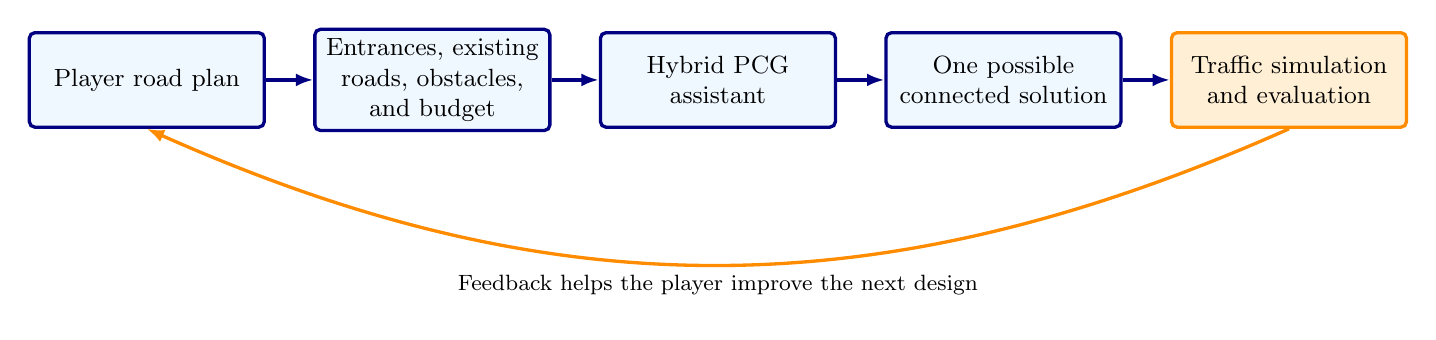
\begin{tikzpicture}[
        node distance=5mm and 6mm,
        flowbox/.style={draw=NavyBlue, rounded corners=2pt, very thick, fill=AliceBlue,
            align=center, minimum height=12mm, text width=2.75cm, font=\small},
        feedback/.style={draw=DarkOrange, rounded corners=2pt, very thick, fill=PapayaWhip,
            align=center, minimum height=12mm, text width=2.75cm, font=\small},
        flowarrow/.style={-{Latex[length=2.2mm]}, very thick, draw=NavyBlue}
    ]
        \node[flowbox] (plan) {Player road plan};
        \node[flowbox, right=of plan] (constraints) {Entrances, existing roads, obstacles, and budget};
        \node[flowbox, right=of constraints] (pcg) {Hybrid PCG assistant};
        \node[flowbox, right=of pcg] (answer) {One possible connected solution};
        \node[feedback, right=of answer] (evaluate) {Traffic simulation and evaluation};

        \draw[flowarrow] (plan) -- (constraints);
        \draw[flowarrow] (constraints) -- (pcg);
        \draw[flowarrow] (pcg) -- (answer);
        \draw[flowarrow] (answer) -- (evaluate);
        \draw[flowarrow, draw=DarkOrange] (evaluate.south) to[bend left=24]
            node[below, font=\footnotesize, align=center] {Feedback helps the player improve the next design}
            (plan.south);
    \end{tikzpicture}
    \caption{The PCG feature supports a player decision loop rather than replacing the player with a final optimal answer.}
    \label{fig:critical-loop}
\end{figure*}

The project also shows a limit of pure L-systems. Local rules can create organic patterns, but they do not understand global connectivity by themselves. Combining local growth with path planning and graph validation was therefore an important design decision.

\section{Testing \& Debugging Summary}

Testing used repeated manual play sessions, Windows builds, runtime logs, cheat commands, and visual debug tools. Tests covered road placement, four building rotations, doorway positions, different seeds and budgets, shared-component connectivity, three difficulty settings, intersection reservations, localisation, tutorial entries, and scoring. A large formal unit-test suite has not yet been completed, which is a current limitation.

Several bugs caused design changes. The first PCG version could report success when buildings belonged to separate road components. Graph-component checks and reserved complete paths fixed this. Rotated rectangular buildings used the rotated size twice, so their visible footprint was wrong. Local mesh size is now separated from the rotated logical footprint. Random odd and even grid sizes also caused half-cell shifts. A stable centre anchor and visualiser redraw fixed this.

A vehicle could also pause when its building entrance was a junction. It first spawned inside the junction collision box before its route direction was ready. The system then marked that junction as already passed. Vehicles now spawn at the first spline point inside the building, and a junction is marked as passed only after a valid entry.

\begin{figure*}[t]
    \centering
    \begin{minipage}[t]{0.32\textwidth}
        \centering
        \includegraphics[height=2.8cm,width=\linewidth,keepaspectratio]{\detokenize{images/Grid and rotated-building alignment before the fix.png}}\\[-1mm]
        \footnotesize (a) Rotated footprint error
    \end{minipage}\hfill
    \begin{minipage}[t]{0.32\textwidth}
        \centering
        \includegraphics[height=2.8cm,width=\linewidth,keepaspectratio]{\detokenize{images/Before image of the procedural sidewalk.png}}\\[-1mm]
        \footnotesize (b) Reversed winding
    \end{minipage}\hfill
    \begin{minipage}[t]{0.32\textwidth}
        \centering
        \includegraphics[height=2.8cm,width=\linewidth,keepaspectratio]{\detokenize{images/After image of the procedural sidewalk.png}}\\[-1mm]
        \footnotesize (c) Unsafe corner inset
    \end{minipage}
    \caption{Visual debugging exposed differences between the logical grid and generated geometry.}
    \label{fig:debug}
\end{figure*}

Figure~\ref{fig:debug} records two stages of the sidewalk fix rather than a false final comparison. Reversed triangle winding first produced a black surface. The next version exposed an inset polygon that folded at rounded corners. Convexity checks and a safe inset limit were then added.

\section{Conclusion}

CityFlow applies research on procedural road generation to a playable planning game. Its main result is a hybrid system that combines player arterial roads, L-system-inspired growth, and connectivity-aware path planning. Traffic, scoring, tutorials, localisation, audio, and visual feedback turn this system into a complete game loop.

Future work should add automated tests for rotation, connectivity, and budget rules. More playtest data would support difficulty tuning. The generator could also compare several valid connection plans and select one by travel time or visual quality.

\printbibliography[title={Bibliography}]

\end{document}
